% !TeX TXS-program:compile = txs:///pdflatex/[--shell-escape]

\documentclass[11pt, letterpaper]{article}

\usepackage{minted}
\usepackage[utf8]{inputenc}
\usepackage[T1]{fontenc}
\usepackage{lmodern}
\usepackage{graphicx}
\usepackage{longtable}
\usepackage{wrapfig}
\usepackage{rotating}
\usepackage{amsmath}
\usepackage{textcomp}
\usepackage{amssymb}
\usepackage{hyperref}
\usepackage[spanish]{babel}
\usepackage[round]{natbib}
\usepackage{subcaption}


\title{\bfseries Tarea}
\author{Ángel García Báez}
\date{\today}
\setcounter{tocdepth}{3} 

\begin{document}
	
	% Página de presentación
	\begin{titlepage}
		\centering
		
\includegraphics[width=0.2\textwidth]{logo.png}\par
		\vspace{1cm}
		{\LARGE \bfseries Universidad Veracruzana \par}
		\vspace{1cm}
		{\Large Maestría en Inteligencia Artificial\par}
		\vspace{3cm}
		{\LARGE \bfseries Visión por Computadora \par}
		\vspace{1cm}
		{\Large \bfseries Tarea 2. Propuesta de implementación del filtro bilineal y del filtro por vecinos más cercanos para el re-escalado de imágenes en Julia. \par}
		\vfill
		{\Large \textit{Ángel García Báez}\par}
		\vspace{1cm}
		{\Large Profesor: Dr. Héctor Acosta Mesa\par}
		\vfill
		{\Large \today \par}
	\end{titlepage}
	
	% Página exclusiva para la tabla de contenidos
	\newpage
	\tableofcontents
	\newpage
	
	% Sección para el problema 1
	\section{Objetivo de la práctica}
	
	El objetivo de la presente practica es crear un programa (en el lenguaje que se prefiera) que sea capaz de hacer zoom para ampliar y achicar una imagen mediante las técnicas de la interpolación bilineal y la interpolación por medio del vecino más cercano.
			
	\begin{figure}[h]
		\centering
		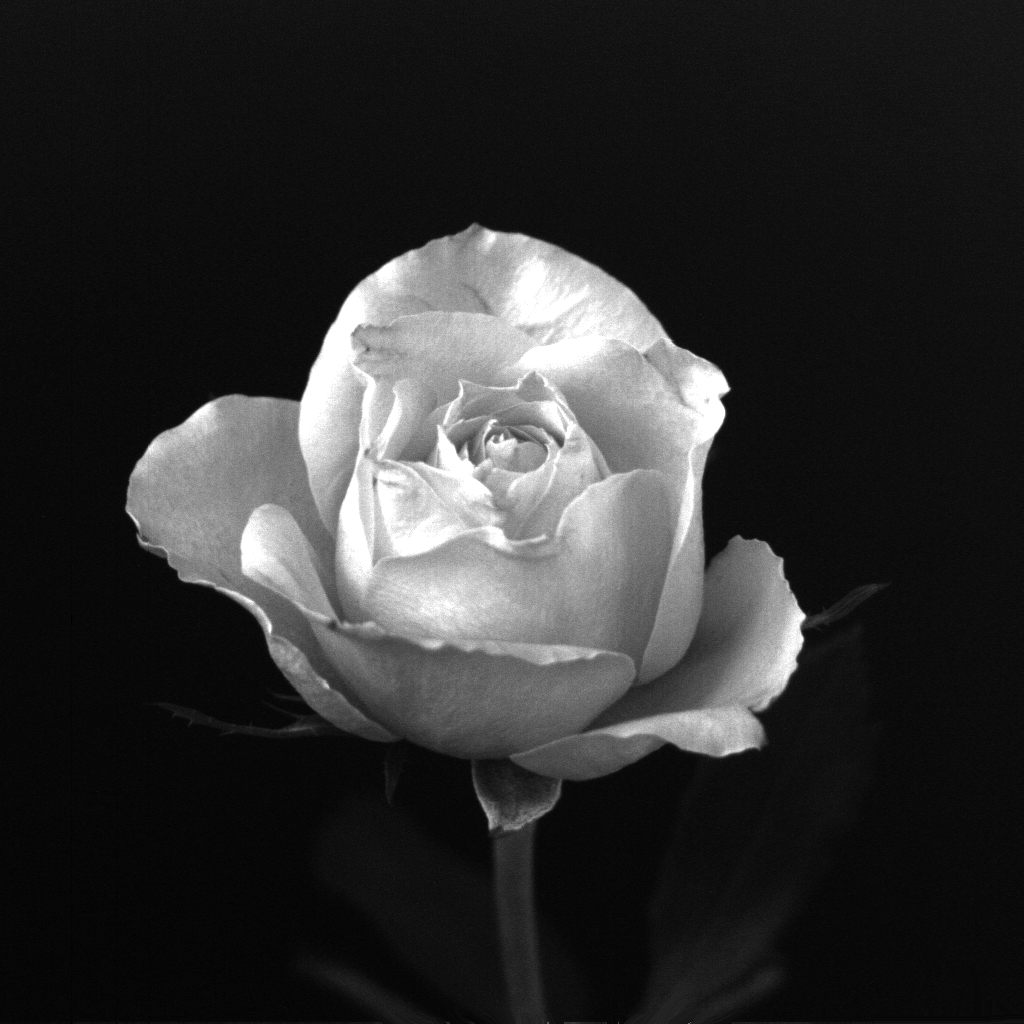
\includegraphics[width=0.7\textwidth]{IMG/Fig2.19(a).jpg}
		\caption{Rosa en escala de grises.}
		\label{fig:f1}
	\end{figure}
	
	Una vez escrito el programa, se hará uso de la imagen mostrada en la figura~\ref{fig:f1} que tiene un tamaño de 1024x1024 pixeles, dicha imagen sera reducida a 256x256 pixeles y posteriormente, sera aumentada desde 256x256 a 1024x1024 pixeles nuevamente. Dicho proceso se aplicara cada uno de las técnicas de interpolado. 
	
	
	\newpage
	
	\section{Metodología}

	Se hará la implementación de las interpolaciones para el re-escalado de las imagenes, siguiendo lo que dice en el libro de \cite{gonzalez2018digital}
	
	\subsection{Interpolacion por vecino más cercano}
	
	El método de interpolación por vecinos más cercanos asigna el valor del píxel más cercano de la imagen original a la imagen escalada. La relación entre las coordenadas \( (x', y') \) en la imagen escalada y las coordenadas \( (x, y) \) en la imagen original se describe mediante las siguientes ecuaciones:
	
	\begin{equation}
		x = \left\lfloor \frac{x' \cdot W}{W'} \right\rfloor
	\end{equation}
	
	\begin{equation}
		y = \left\lfloor \frac{y' \cdot H}{H'} \right\rfloor
	\end{equation}
	
	Donde \( W \) y \( H \) son las dimensiones de la imagen original, y \( W' \) y \( H' \) son las dimensiones de la imagen escalada. El valor del píxel \( I(x, y) \) de la imagen original se asigna al píxel correspondiente en la imagen escalada \( I'(x', y') \):
	
	\begin{equation}
		I'(x', y') = I(x, y)
	\end{equation}
	
	\subsection{Interpolación Bilineal}
	
	La interpolación bilineal se utiliza para estimar el valor de un píxel en una imagen escalada basado en sus vecinos más cercanos en una imagen original. Se fundamenta en la interpolación lineal en dos direcciones: horizontal y vertical.
	
	Dado un punto $(X, Y)$ en la imagen escalada, su posición en la imagen original se encuentra mediante la relación:
	
	\begin{equation}
		X = \frac{x' (W - 1)}{W'} + 1, \quad Y = \frac{y' (H - 1)}{H'} + 1
	\end{equation}
	
	donde:
	- $(x', y')$ son las coordenadas en la imagen escalada.
	- $(W', H')$ son las dimensiones de la imagen escalada.
	- $(W, H)$ son las dimensiones de la imagen original.
	
	Los cuatro píxeles vecinos en la imagen original se ubican en:
	
	\begin{equation}
		(x_1, y_1), \quad (x_2, y_1), \quad (x_1, y_2), \quad (x_2, y_2)
	\end{equation}
	
	donde:
	\begin{align*}
		x_1 &= \lfloor X \rfloor, \quad x_2 = \min(x_1 + 1, W) \\
		y_1 &= \lfloor Y \rfloor, \quad y_2 = \min(y_1 + 1, H)
	\end{align*}
	
	Los valores de intensidad de los píxeles vecinos se denotan como:
	
	\begin{equation}
		Q_{11} = I(x_1, y_1), \quad Q_{21} = I(x_2, y_1), \quad Q_{12} = I(x_1, y_2), \quad Q_{22} = I(x_2, y_2)
	\end{equation}
	
	La interpolación bilineal se obtiene mediante la siguiente ecuación:
	
	\begin{equation}
		I(X, Y) = (1 - d_x)(1 - d_y) Q_{11} + d_x (1 - d_y) Q_{21} + (1 - d_x) d_y Q_{12} + d_x d_y Q_{22}
	\end{equation}
	
	donde:
	
	\begin{align*}
		d_x &= X - x_1 \\
		d_y &= Y - y_1
	\end{align*}
	
	Estos coeficientes representan la distancia relativa entre el punto interpolado y los píxeles originales. Finalmente, el valor resultante $I(X, Y)$ se redondea para obtener un valor discreto en la imagen escalada.
	
	\newpage
	
	\section{Resultados}
	
	Tras la implementación del código, se muestran los resultados por tipo de filtro:
	
	\subsection{Interpolacion bilineal}
	
	\begin{figure}[h]
		\centering
		% Imagen de la izquierda (b1.jpg)
		\begin{minipage}{0.45\textwidth}
			\centering
			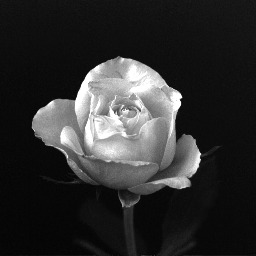
\includegraphics[width=\textwidth]{IMG/b1.jpg}
			\caption{Imagen original reescalada a 256x256.}
			\label{fig:b1}
		\end{minipage}
		\hfill
		% Imagen de la derecha (b2.jpg)
		\begin{minipage}{0.45\textwidth}
			\centering
			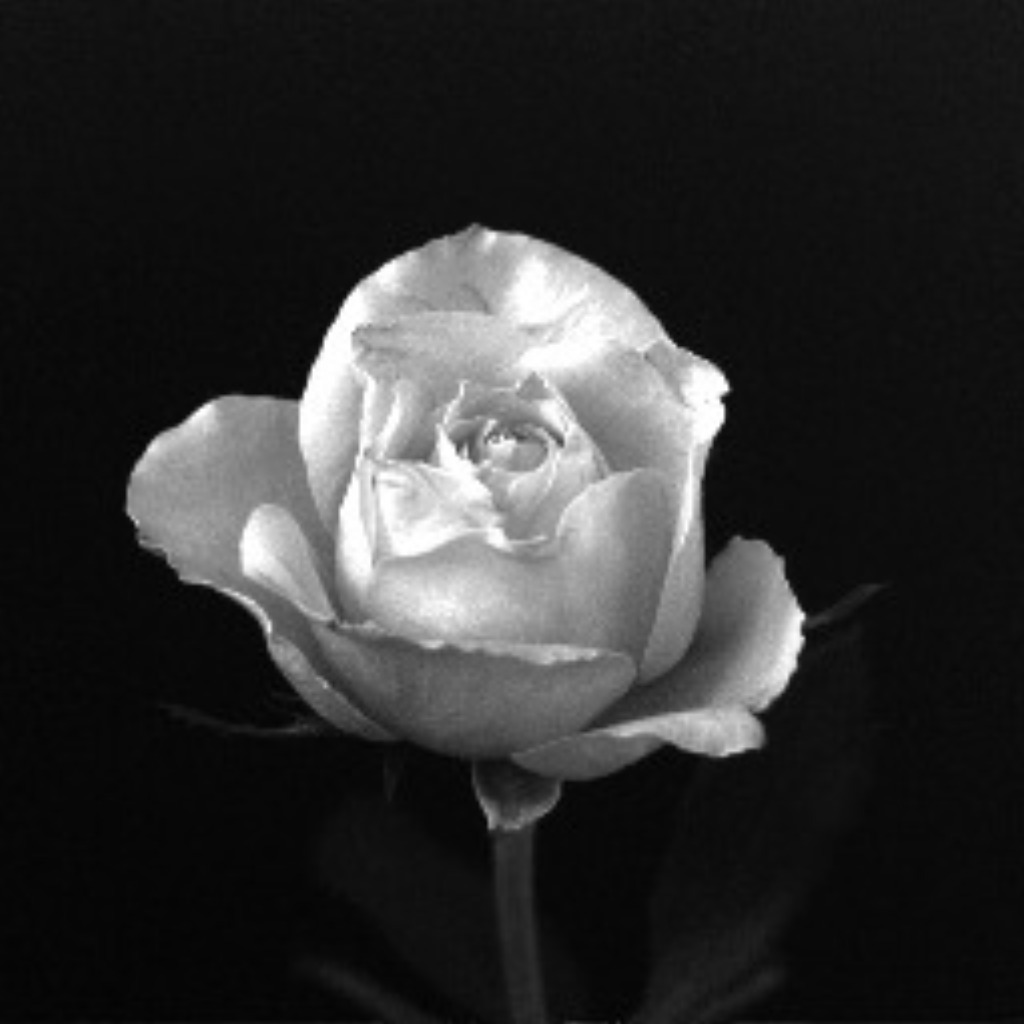
\includegraphics[width=\textwidth]{IMG/b2.jpg}
			\caption{Imagen de 256x256 reescalada a 1024x1024.}
			\label{fig:b2}
		\end{minipage}
		\caption{Comparación entre la imagen original reescalada a 256x256 y la versión ampliada a 1024x1024 mediante la interpolación bilineal.}
		\label{fig:comparacion}
	\end{figure}

	Se observa que a simple vista existe poca diferencia entre una imagen y otra, podrían parecer la misma si se mira por encima, sin embargo, al aplicar zoom sobre ellas, se logra apreciar como la imagen de la izquierda muestra sus pixeles de forma más evidente que la imagen de la derecha.
	
	%%%% Segundos resultados	
	\newpage
	
	
	\subsection{Interpolacion por vecino más cercano}
	
	\begin{figure}[h]
		\centering
		% Imagen de la izquierda (b1.jpg)
		\begin{minipage}{0.45\textwidth}
			\centering
			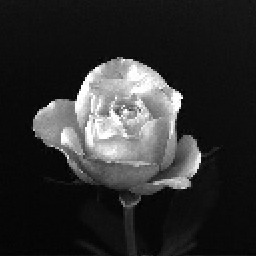
\includegraphics[width=\textwidth]{IMG/v1.jpg}
			\caption{Imagen original reescalada a 256x256.}
			\label{fig:b1}
		\end{minipage}
		\hfill
		% Imagen de la derecha (b2.jpg)
		\begin{minipage}{0.45\textwidth}
			\centering
			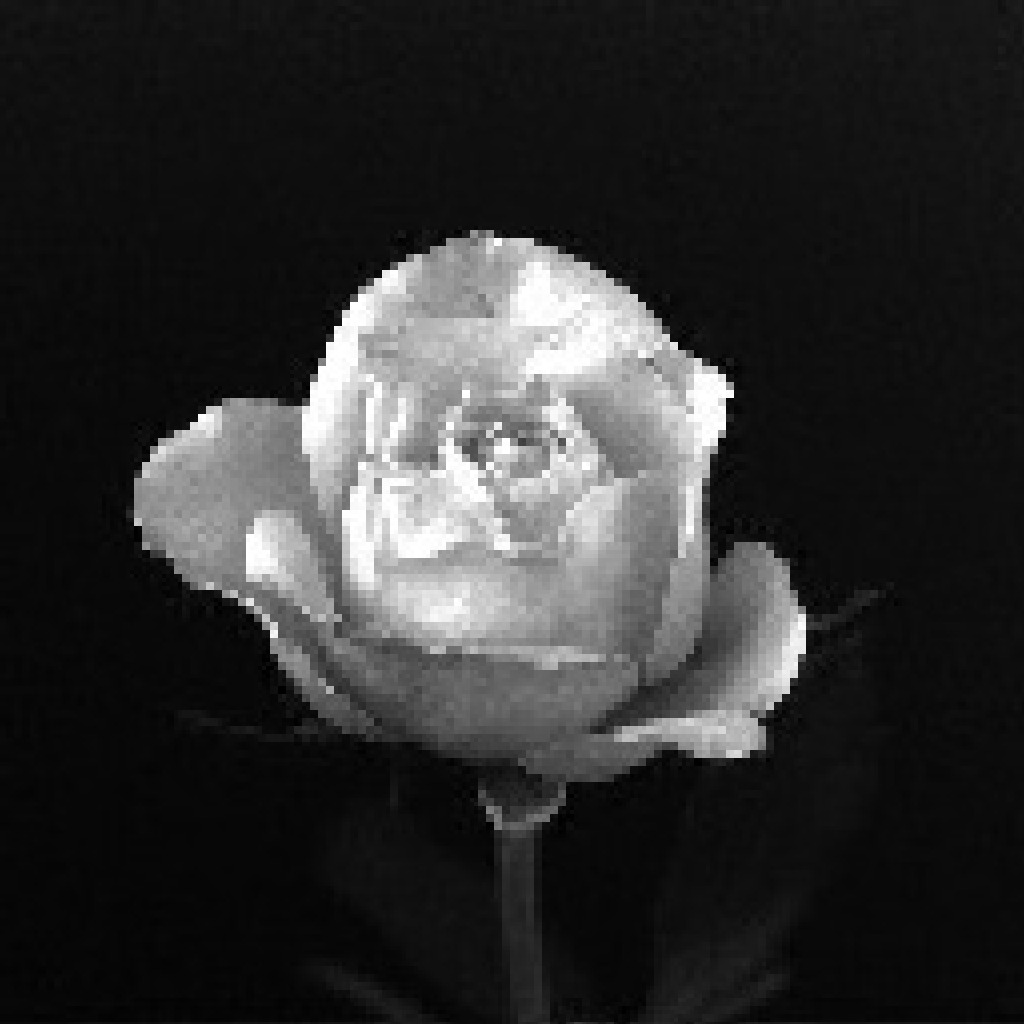
\includegraphics[width=\textwidth]{IMG/v2.jpg}
			\caption{Imagen de 256x256 reescalada a 1024x1024.}
			\label{fig:b2}
		\end{minipage}
		\caption{Comparación entre la imagen original reescalada a 256x256 y la versión ampliada a 1024x1024 mediante la interpolación del vecino más cercano.}
		\label{fig:comparacion}
	\end{figure}
	
	En la imagen de la izquierda se observa una evidente baja en la resolución, puesto que los pixeles se ven a simple vista, como si fuera una imagen sacada de un videojuego viejito. Por otro lado, la imagen de la derecha, al intentar ser re-escalada desde una imagen tan pixelada, arrastra consigo esta perdida de calidad al ser aumentada, lo que hace más evidente que la imagen no se vea tan suave.
	

	\newpage

	
	\section{Conclusiones}
	
	Tras lo observado en los resultados, es evidente que la interpolación por medio de los vecinos más cercanos es más "simple" de implementar pero esa simpleza, se nota en los resultados que produce, dado que al tomar los primeros pixeles que encuentra, hace que no exista un cambio suave o gradual entre los colores que hacen evidente la baja resolución de la imagen al mostrarse tan pixelada. Dicho comportamiento lo mantiene tanto al reducir imágenes como aumentarlas, puesto que al aumentar las imágenes bajo dicho mecanismo, hace que los pixeles crezcan, haciendo que la imagen siga pareciendo de baja resolución pero en un tamaño mayor.
	
	Por otro lado, el filtro bilineal que es producto de un proceso más refinado y en cierta medida, más complejo de implementar respecto al anterior, produce imagenes más suaves en el sentido de que al bajar la resolución de la imagen, no se nota de primeras el como se pixela la imagen de primeras, es hasta que se le hace un zoom que se observan dichos detalles. Este método logra re-escalar bien la imagen de modo que casi pareciera que se reconstruye la imagen original de manera fidedigna.

	\newpage

	
\section{Referencias}  % Sección numerada de referencias

\bibliographystyle{apalike}  % Estilo de citas (puedes cambiarlo)
\bibliography{Biblio}        % Nombre del archivo BibTeX (sin extensión)

	\newpage
	
	\section{Anexos}


	
	\subsection{Implementación de los filtros}
	
	
\begin{itemize}
	\begin{minted}[linenos,firstnumber=1]{julia}
#### Interpolación bilineal ####
		
# Definir el filtro bilineal
# Parametros de entrada: 
## Imagen de entrada
## Ancho de salida
## Alto de salida
function bilineal(Imagen,Ancho,Alto) 
	# Parametros de salida de la nueva matriz #
	naltura = Ancho
	nancho = Alto
	# Crear la nueva matriz de enteros de tamaño naltura X nancho
	nueva = zeros(Int,naltura,nancho);
	#### Dmensiones originales de la matriz
	Oaltura = size(Imagen)[1]
	Oancho = size(Imagen)[2]
	#### Definir la relación entre los tamaños
	escalaX = (Oancho-1)/(nancho-1);
	escalaY = (Oaltura-1)/(naltura-1);
	#### Aplicación del escalado ####
	for i in 1:naltura
		# Segundo loop
		for j in 1:nancho
			# Coordenadas de la imagen original
			X = escalaX*(j-1) + 1 # Adelante del borde
			Y = escalaY*(i-1) + 1 # Adelante del borde
			### Datos para hacer el interpolado ###
			## Coordenadas en X ##
			x1 = floor(Int,X)
			x2 = min(x1+1,Oancho)
			## Coordenadas en Y ##
			y1 = floor(Int,Y)
			y2 = min(y1+1,Oaltura)
			# Pesos para la interpolación #
			dx = X-x1
			dy = Y-y1
			### Extraer los valores de los pixeles vecinos ####
			Q11 = Imagen[y1,x1]
			Q12 = Imagen[y2,x1]
			Q21 = Imagen[y1,x2]
			Q22 = Imagen[y2,x2]
			### Crear el pixel con la interpolación ####
			px = (1-dx)*(1-dy)*Q11 +
			dx*(1-dy)*Q21 +
			(1-dx)*dy*Q12 +
			dx*(dy)*Q22
			# Guardarlo en la matriz de salida #
			nueva[i,j] = round.(Int,px)
		end
	end
	# Devolver la matriz resultante
	# Convertir en escala de grises #
	res = clamp.(nueva./255,0,1);
	# Convertir la matriz en escala de grises
	return(Gray.(res)) 
end
		
#### Interpolación del vecino más cercano ####	
# Función de interpolación por vecinos más cercanos
function vecinos(Imagen, Ancho, Alto)
	# Dimensiones de la nueva imagen
	naltura = Alto
	nancho = Ancho
	# Crear la nueva matriz de enteros de tamaño naltura × nancho
	nueva = zeros(Int, naltura, nancho)
		
	# Dimensiones originales de la imagen
	Oaltura, Oancho = size(Imagen)
		
	# Relación de escalado
	escalaX = Oancho / nancho
	escalaY = Oaltura / naltura
		
	# Aplicar el escalado con vecinos más cercanos
	for i in 1:naltura
		for j in 1:nancho
			# Coordenadas en la imagen original
			X = round(Int, escalaX * (j - 0.5))  # Píxel más cercano en X
			Y = round(Int, escalaY * (i - 0.5))  # Píxel más cercano en Y
		
			# Asegurar que las coordenadas estén dentro del rango
			X = clamp(X, 1, Oancho)
			Y = clamp(Y, 1, Oaltura)
		
			# Asignar el valor del píxel más cercano
			nueva[i, j] = Imagen[Y, X]
		end
	end
		
	# Convertir en escala de grises y normalizar
	res = clamp.(nueva ./ 255, 0, 1)
	return Gray.(res)
end
		

#### Cargar la imagen de la rosa ####
# Cargar las librerias para el procesado de imagenes
using Images
#using ImageView
# Imagen De referencia
ruta = "IMG/Fig2.19(a).jpg"
img = load(ruta)
img1 = Gray.(img)
# Guardar la imagenm
#save("IMG/IM1gray.jpg", img1)
		
### Pruebas para el filtro bilieal ###
#### Re escalar la imagen original a 256x256 pixeles ####
		
# Imagen De referencia
img1 = round.(Int,Gray.(img).* 255)
res1 = bilineal(img1,256,256)
save("IMG/b1.jpg", res1) #  Guardar el resultado
res1
		
#### Re escalar la imagen de 256x256 pixeles a 1024x1024 ####
# Imagen De referencia
ruta1 = "IMG/b1.jpg"
img = load(ruta1)
img2 = round.(Int,Gray.(img).* 255)
res2 = bilineal(img2,1024,1024)
save("IMG/b2.jpg", res2) #  Guardar el resultado
res2
		
### Pruebas para el filtro del vecino más cercano ###
#### Re escalar la imagen original a 256x256 pixeles ####
		
# Imagen De referencia
img3 = round.(Int,Gray.(img).* 255)
res3 = vecinos(img3,256,256)
save("IMG/v1.jpg", res3) #  Guardar el resultado
res3
		
#### Re escalar la imagen de 256x256 pixeles a 1024x1024 ####
# Imagen De referencia
ruta2 = "IMG/v1.jpg"
img = load(ruta2)
img4 = round.(Int,Gray.(img).* 255)
res4 = vecinos(img4,1024,1024)
save("IMG/v2.jpg", res4) #  Guardar el resultado
res4
	\end{minted}
\end{itemize}

	
	
	
	
	
	
	
\end{document}

